\message{ !name(VoorstudieFase1.tex)}\documentclass[12pt]{report}

\usepackage[utf8]{inputenc}
\usepackage[dutch]{babel}
\usepackage{graphicx}
\usepackage{titlesec}
\usepackage{etoolbox}
\usepackage{parskip}
\usepackage{hyperref}
\usepackage{amssymb}
\usepackage[table,xcdraw]{xcolor}
\usepackage{tikz}

\usetikzlibrary{arrows,automata}
\usetikzlibrary{positioning}

\selectlanguage{dutch}

\graphicspath{{images/}}

\titleformat
{\chapter}
[hang]
{\bfseries\huge}
{\thechapter\quad}
{0.2ex}{}[]

\titlespacing{\chapter}{1pc}{1ex minus 5ex}{1pc}

\makeatletter
\patchcmd{\chapter}{\if@openright\cleardoublepage\else\clearpage\fi}{}{}{}
\makeatother


\tikzset{
    state/.style={
           rectangle,
           rounded corners,
           draw=black, very thick,
           minimum height=2em,
           inner sep=3pt,
           text centered,
           },
}

\title{{Programmeerproject 1:}\\
				{FireAnt}\\
				{\large Fase 1}}
\author{{Erneste Richard Rwema Rugema}\\
    {(erneste.richard.rwema.rugema@vub.be)}\\
			{\leftmark rolnummer: 0580198}}
\date{Academiejaar 2021-2022}

\begin{document}

\message{ !name(VoorstudieFase1.tex) !offset(-3) }


\maketitle

\tableofcontents
\newpage

\chapter{Intorductie}
Dit document beschrijft het implementatie in fase 1 van het spel \texttt{Fire Ant} in scheme \textbf{r5rs}.
Het maakt deel uit van het opleidingsonderdeel "Programmeerproject 1".

\section{Spelbeschrijving}
In dit spel is het de bedoeling dat een speler een \textit{vuurmier} bestuurt,
die tracht zijn mierenkoningin te redden van schorpioenenleger.
Om dit te voltooien moet de speler een serie van levels, die toenemen in moeilijkheidsgraad,
oplossen zodat hij tot bij de koningin geraakt.
Een level bestaat uit een doolhof gevuld met puzzels, items en vijanden.
Enkel door deze puzzels op te lossen en de schorpioenen te vermijden, kan de speler het level oplossen.
Het spel eindigt dan tot dat alle levels opgelost zijn of tot dat de speler al zijn levens verloren heeft.

\section{Implementatie}
Voor het eerste fase zal het genoeg zijn om de elementaire elementen van het spel te implementeren.

Onder andere:
\begin{itemize}
	\item Het spel maakt een spelwereld met een doolhof waarin een vuurmier, die door de speler kan bestuurt worden, kan rond lopen.
	\item Het doolhof bevat ook (een) schorpioen(en) die een vaste pad aflegt.
	\item	De vuurmier moet bij aanraking van de schorpioen terug naar zijn start positie gaan.
	\item Verspreid doorheen het doolhof moeten er verschillenden eitjes geplaatst zijn,
		die vuurmier kan oprapen.
\end{itemize}

Het programma zal ook verdeelt worden uit
een controller (zal tussen de modellen en views moeten communiceren)
modellen (bezitten al de spellogica)
en de views (zorgt voor het tekenlogica van het spel)



\chapter{ADTs}
In deze sectie zullen alle ADTs en hun proceduren beschreven worden 
die in het programma voorkomen.
Deze ADTs zullen verdeelt worden in 3 categorieën:
\nameref{controller},
\nameref{model} en
\nameref{view}
%%%%%%%%%%%%%%%%%%%%%%%%%%%%% CONTROLLER %%%%%%%%%%%%%%%%%%%%%%%%%%%%%%%%%%
\section{Controller}
\label{controller}
De controller zal centraal zijn om de interacties tussen de modellen en views te beheren. 

\subsection{Game ADT}
\label{section:game}
Het \texttt{\nameref{section:game}} is het centrale ADT dat het spel opstart en beheert.
Deze is verantwoordelijk voor
het initialiseren van de \texttt{\nameref{section:player}},
het initialiseren en starten van de juiste \texttt{\nameref{section:level}},
het verwerken van de speler invoer
en het behandelen van het spellus.

\begin{table}[hbt]
\centering
\begin{tabular}{|ll|}
\hline
\rowcolor[HTML]{000000} 
{\color[HTML]{FFFFFF} \textbf{Naam}} & {\color[HTML]{FFFFFF} \textbf{Signatuur}} \\ \hline
new-game    & $($list $\rightarrow$ Game$)$                  \\ \hline
start       & $(\varnothing \rightarrow \varnothing)$        \\ \hline
next-level! & $(\varnothing \rightarrow \varnothing)$     	 \\ \hline
key-handler & $($symbol symbol $\rightarrow \varnothing)$    \\ \hline
game-loop   & $($number $\rightarrow \varnothing)$           \\ \hline
\end{tabular}
\caption{Operaties van het \texttt{\nameref{section:game}}}
\label{table:1}
\end{table}

Het \texttt{\nameref{section:game}} bevat de volgende operaties:

\begin{itemize}
	\item \textbf{new-game}: Deze operatie maakt een object van het \texttt{\nameref{section:game}} aan.
	\item \textbf{start}: Start een nieuw spel op.
		Eerst slaagt het alle namen van de levels (dit zijn csv bestanden) uit de "level" map op, in een lijst.
		Deze lijst gebruikt het om de eerste \texttt{\nameref{section:level}} object te maken.
		Vervolgens maakt het een nieuwe object van het \texttt{\nameref{section:player}} en het \texttt{\nameref{section:view}}.
		Tenslotte "start" het, de spellus en gebruikers invoer met behulp van de game-loop en key-handler procedures respectievelijk. 
	\item \textbf{next-level!}: Veranderd de huidige level (current-level) naar de volgende level in de levels lijst.
		De oude level wordt ook verwijderd uit de levels lijst.
		Het update ook de huidige level van de \texttt{\nameref{section:view}}.
	\item \textbf{key-handler}: Neemt twee argumenten op state en key.
		State is de status van de toets (key) op het huidige moment.
		Op dit moment ondersteunt de functie enkel de pijltjes toetsen ingedrukt.
		Wanneer dit gebeurt, beweegt het respectievelijk de speler als deze niet tegen een muur aanloopt.
	\item \textbf{game-loop}: Neemt een argument op ms (milliseconde voor vorige aanroep).
		Als de huidige level niet uitgespeeld is dan
		update het de huidige level en de view object.
		Daarnaast als de speler sterft, herleeft de level, de speler opnieuw.
		In het geval dat het huidige level uitgespeeld is voer het next-level procedure op.
\end{itemize}

%%%%%%%%%%%%%%%%%%%%%%%%%%%%%% MODELLEN %%%%%%%%%%%%%%%%%%%%%%%%%%%%%%%%%%%
\section{Modellen}
\label{model}
De Modellen zullen verantwoordelijk zijn voor het spellogica m.a.w. alle berekening achter de schermen.

\section{Level ADT}
\label{section:level}
Het \texttt{\nameref{section:level}} is het ADT dat een level opbouwt aan de hand van csv tekst bestand.
Deze is verantwoordelijk om
een csv bestand te lezen en zijn elementen ervan te interpreteren,
het onthouden en aanmaken van alle nodige objecten in de level (bv. schorpioenen, eiren, het doolhof, etc.),
de speler te laten herstarten,
het updaten van de elementen in de level,
het onthouden van de startpositie (spawn)
en te checken of het level is uitgespeeld.

\begin{table}[hbt]
\centering
\begin{tabular}{|ll|}
\hline
\rowcolor[HTML]{000000} 
{\color[HTML]{FFFFFF} \textbf{Naam}} & {\color[HTML]{FFFFFF} \textbf{Signatuur}} \\ \hline
new-level      & (Player string $\rightarrow$ Level)   \\ \hline
init           & (string $\rightarrow$ $\varnothing$)                      \\ \hline
get-maze       & ($\varnothing$ $\rightarrow$ Maze)                        \\ \hline
get-eggs       & ($\varnothing$ $\rightarrow$ list)                        \\ \hline
get-scorpions  & ($\varnothing$ $\rightarrow$ list)                        \\ \hline
get-updates    & ($\varnothing$ $\rightarrow$ list)                        \\ \hline
is-finished?   & (Player $\rightarrow$ boolean)                            \\ \hline
is-legal-move? & (Object\footnotemark{} symbol $\rightarrow$ boolean)      \\ \hline
update!        & ($\varnothing$ $\rightarrow$ $\varnothing)$               \\ \hline
respawn        & ($\varnothing$ $\rightarrow$ $\varnothing$)               \\ \hline
on-collision   & ((Object\footnotemark[\value{footnote}] $\rightarrow$ $\varnothing$) $\rightarrow$ $\varnothing$) \\ \hline
interpret!     & (string number number $\rightarrow$ $\varnothing$)        \\ \hline
\end{tabular}
\caption{Operaties van het \texttt{\nameref{section:level}}}
\label{table:level}
\end{table}


Het \texttt{\nameref{section:level}} bevat de volgende operaties:
\begin{itemize}
	\item \textbf{new-level}: Neemt een \texttt{\nameref{section:level}} en de naam van level csv bestand op als argument op.
		Deze procedure geeft een object van het type level terug.
		Deze level object bezit alle elementen die het level bezit.
	\item \textbf{init}: Deze procedure initialiseert het level door de element van het csv bestaand een na een door te geven aan het interpret! procedure
		met de x en y positie van de element in de csv bestand.
	\item \textbf{get-maze}: Geeft de \texttt{\nameref{section:maze}} object terug opgeslagen in de \texttt{\nameref{section:level}}.
	\item \textbf{get-eggs}: Geeft een lijst van \texttt{\nameref{section:egg}} objecten terug die opgeslagen zijn in de \texttt{\nameref{section:level}}.
	\item \textbf{get-scorpions}: Geeft een lijst van \texttt{\nameref{section:scorpion}} objecten terug die opgeslagen zijn in de \texttt{\nameref{section:level}}.
	\item \textbf{get-updates}: Geeft een lijst van objecten terug die in de huidige iteratie van de spellus geüpdatet zijn.
	\item \textbf{is-finished?}: Geeft aan of het spel is uitgespeeld door te kijken of de \texttt{\nameref{section:player}} helemaal onderaan de doolhof is geraakt.
	\item \textbf{is-legal-move?}: Neemt een Object (dat een \texttt{\nameref{section:positie}} bezit) en een direction ('up, 'down, 'left or 'right) als argument op.
		Het zoekt met met behulp van de positie van het Object naar zijn buur positie gelegen op de ``direction''.
		Tenslotte kijkt de functie of de gebuurt positie een muur is aan de hand van de \texttt{\nameref{section:maze}}.
	\item \textbf{update!}: De procedure update de ``updates'' lijst
		door eerst de nodige objecten te updaten (en dus ook toe te voegen aan de lijst).
		Vervolgens checkt het of er objecten zijn die botsen met het Player object 
		en zo ja, voeren ze hun eigen procedure uit 
		(bv. schorpioenen vermoorden de speler en eiren worden genomen/verdwijnen).
		Deze objecten worden dan ook toegevoegd aan de lijst.
	\item \textbf{respawn}: Deze procedure plaatst de Player terug op zijn start positie en geeft hem terug ``leven''.
	\item \textbf{on-collision}: Neemt een procedure (die wordt uitgevoerd als er een botsing met de Player gebeurt) 
		en een lijst van objecten die gecheckt moeten worden voor botsingen met de Player.
	\item \textbf{interpret!}: Deze procedure neemt een string
		(dat een element uit de csv bestand is)
		, een x en y positie (dat de positie van de string voorstelt in de csv bestand).
		Deze warden worden gebruikt om Objecten (zoals een Egg, Scorpion of Start Positie) maken 
		of de \texttt{\nameref{section:maze}} aan te vullen in het \texttt{\nameref{section:level}}.
\end{itemize}

\footnotetext{Object is een object dat een Positie ADT bezit.}

\section{Maze ADT}
\label{section:maze}
Het \texttt{\nameref{section:maze}} is verantwoordelijk om het spellogica van het doolhof te construeren.

\begin{table}[hbt]
\centering
\begin{tabular}{|ll|}
\hline
\rowcolor[HTML]{000000} 
{\color[HTML]{FFFFFF} \textbf{Naam}} & {\color[HTML]{FFFFFF} \textbf{Signatuur}} \\ \hline
new-maze   & ($\varnothing$ $\rightarrow$ Maze)                          \\ \hline
get-type   & ($\varnothing$ $\rightarrow$ symbol)                        \\ \hline
get-height & ($\varnothing$ $\rightarrow$ number)                        \\ \hline
get-width  & ($\varnothing$ $\rightarrow$ number)                        \\ \hline
is-wall?   & (number number $\rightarrow$ boolean)                       \\ \hline
set-wall!  & (number number boolean $\rightarrow$ $\varnothing$)         \\ \hline
\end{tabular}
\caption{Operaties van het \texttt{\nameref{section:maze}}}
\label{table:maze}
\end{table}

Het \texttt{\nameref{section:maze}} bevat de volgende operaties:

\begin{itemize}
	\item \textbf{new-maze}: Deze operatie maakt een object van het \texttt{\nameref{section:maze}} aan.
	\item \textbf{get-type}: Geeft het type van de ADT terug in dit geval 'maze.
	\item \textbf{get-height}: Geeft het hoogte van de doolhof terug.
		Deze is gedefinieerd door het GRID-HEIGHT constante in het ``etc/constante.rkt'' bestand.
	\item \textbf{get-width}: Geeft het hoogte van de doolhof terug.
		Deze is gedefinieerd door het GRID-WIDTH constante in het ``etc/constante.rkt'' bestand.
	\item \textbf{is-wall?}: Checkt of de gegeven rij en kolom een muur is en of de positie bestaat in het \texttt{\nameref{section:maze}}.
	\item \textbf{set-wall!}: Zet of verwijderd een muur 
		(op basis van de gegeven

		boolean warden) in het \texttt{\nameref{section:maze}} op de gegeven rij en kolom.
\end{itemize}

\section{Position ADT}
\label{section:positie}

De \texttt{\nameref{section:positie}} is verantwoordelijk voor het bijhouden en aanpassen van de positie, oriëntatie en snelheid van een object.

\begin{table}[hbt]
\centering
\begin{tabular}{|ll|}
\hline
\rowcolor[HTML]{000000} 
{\color[HTML]{FFFFFF} \textbf{Naam}} & {\color[HTML]{FFFFFF} \textbf{Signatuur}} \\ \hline
new-position     & (number number $\rightarrow$ Positie)                       \\ \hline
get-type         & ($\varnothing$ $\rightarrow$ symbol)                        \\ \hline
get-x            & ($\varnothing$ $\rightarrow$ number)                        \\ \hline
get-y            & ($\varnothing$ $\rightarrow$ number)                        \\ \hline
get-orientation  & ($\varnothing$ $\rightarrow$ symbol $\cup\{\#f\}$)          \\ \hline
get-speed        & ($\varnothing$ $\rightarrow$ number)                        \\ \hline
set-x!           & (number $\rightarrow$ $\varnothing$)                        \\ \hline
set-y!           & (number $\rightarrow$ $\varnothing$)                        \\ \hline
set-orientation! & (symbol $\rightarrow$ $\varnothing$)                        \\ \hline
set-moving!      & (bool $\rightarrow$ $\varnothing$)                          \\ \hline
is-moving?       & ($\varnothing$ $\rightarrow$ boolean)                       \\ \hline
is-colliding?    & (Position $\rightarrow$ boolean)                            \\ \hline
move!            & (symbol $\rightarrow$ $\varnothing$)                        \\ \hline
peek             & (symbol $\rightarrow$ Position)                             \\ \hline
\end{tabular}
\caption{Operaties van het \texttt{\nameref{section:positie}}}
\label{table:positie}
\end{table}

Het \texttt{\nameref{section:positie}} bevat de volgende operaties:

\begin{itemize}
	\item \textbf{new-positie}: Deze operatie maakt een nieuw object van het \texttt{\nameref{section:positie}} aan. 
		Deze neemt 2 nummers op als argument
		dat respectievelijk de x- en y-co\"ordinaat representeren in het \texttt{\nameref{section:maze}}.
	\item \textbf{get-type}: Geeft het type van de ADT terug in dit geval 'position.
	\item \textbf{get-x}: Geeft x positie terug.
	\item \textbf{get-y}: Geeft y positie terug.
	\item \textbf{get-orientation}: Geeft de oriëntatie van het object terug.
		Het is standaard \#f.
	\item \textbf{get-speed}: Geeft de snelheid van het object terug.
		De snelheid in dit context is 
		de snelheid waarmee het spel een tile van 1 positie naar een ander tekent.
		Deze is standaard 0,17.
	\item \textbf{set-x}: Veranderd de x positie door de gegeven nummer.
	\item \textbf{set-y}: Veranderd de y positie door de gegeven nummer.
	\item \textbf{set-orientation}: Veranderd de oriëntatie positie door de gegeven richting.
	\item \textbf{set-moving}: Veranderd boolean waarde van het moving variabel.
		De variabel geeft aan of het object nog steeds aan het bewegen is van zijn vorige positie naar zijn nieuwe positie.
	\item \textbf{is-moving?}: Geeft aan of het object zich nog steeds aan het verplaatsen is naar zijn nieuwe positie.
	\item \textbf{is-colliding?}: Checkt of het meegegeven Positie de zelfde positie heeft in de Maze.
	\item \textbf{move!}: Verandert het positie en oriëntatie van het \texttt{\nameref{section:positie}} in de gegeven richting.
		Zolang deze positie nog niet aan het bewegen is naar een nieuw positie.
	\item \textbf{peek}: Geef de positie terug van buur positie gelegen op de meegegeven richting.
\end{itemize}

\section{Egg ADT}
\label{section:egg}

Het \texttt{\nameref{section:egg}} stelt een voorwerp voor dat kan opgeraapt  worden door een \texttt{Player}.

\begin{table}[hbt]
\centering
\begin{tabular}{|ll|}
\hline
\rowcolor[HTML]{000000} 
{\color[HTML]{FFFFFF} \textbf{Naam}} & {\color[HTML]{FFFFFF} \textbf{Signatuur}} \\ \hline
new-egg                              & (Positie $\rightarrow$ Egg) \\ \hline
get-type         & ($\varnothing$ $\rightarrow$ symbol)                        \\ \hline
get-position         & ($\varnothing$ $\rightarrow$ Position)                        \\ \hline
take!                              & ($\varnothing$ $\rightarrow$ $\varnothing$)                   \\ \hline
is-taken?                         & ($\varnothing$ $\rightarrow$ boolean)               \\ \hline
\end{tabular}
\caption{Operaties van het \texttt{\nameref{section:egg}}}
\label{table:item}
\end{table}

Het \texttt{\nameref{section:egg}} bevat de volgende operaties:

\begin{itemize}
	\item \textbf{new-egg}: Maakt een nieuw object van het \texttt{\nameref{section:egg}}.
	\item \textbf{get-type}: Geeft het type van de ADT terug in dit geval 'egg.
	\item \textbf{get-position}: Geeft het \texttt{\nameref{section:positie}} object terug die het egg object bezit.
	\item \textbf{take!}: Veranderd taken waarden naar \#t.
		Met andere worden het egg is opgerapen.
	\item \textbf{is-taken?}: Check of het \texttt{\nameref{section:egg}} is opgeraapt of niet.
\end{itemize}

\section{Player ADT}
\label{section:player}
De \texttt{\nameref{section:player}} stelt het speler voor.
Deze ADT is verantwoordelijk om de conditie van de speler bij te houden.
Met andere woorden zijn aantal levens, zijn positie en de huidige leven conditie van de speler.

\begin{table}[hbt]
\centering
\begin{tabular}{|ll|}
\hline
\rowcolor[HTML]{000000} 
{\color[HTML]{FFFFFF} \textbf{Naam}} & {\color[HTML]{FFFFFF} \textbf{Signatuur}} \\ \hline
new-player    & ($\varnothing$ $\rightarrow$ Player) \\ \hline
get-type      & ($\varnothing$ $\rightarrow$ symbol)                        \\ \hline
get-position  & ($\varnothing$ $\rightarrow$ Position $\cup\{\#f\}$)                        \\ \hline
set-position! & (Position $\rightarrow$ $\varnothing$)                        \\ \hline
is-dead?      & ($\varnothing$ $\rightarrow$ boolean)               \\ \hline
die!          & ($\varnothing$ $\rightarrow$ $\varnothing$)                   \\ \hline
revive!       & ($\varnothing$ $\rightarrow$ $\varnothing$)                   \\ \hline
\end{tabular}
\caption{Operaties van het \texttt{\nameref{section:player}}}
\label{table:ant}
\end{table}

De \texttt{\nameref{section:player}} bevat de volgende operaties:

\begin{itemize}
	\item \textbf{new-player}: Maakt een object van \texttt{\nameref{section:player}} aan.
	\item \textbf{get-type}: Geeft het type van de ADT terug in dit geval 'player.
	\item \textbf{get-position}: Geeft de \texttt{\nameref{section:player}} object terug die het player object bezit.
	\item \textbf{set-position!}: Geeft de \texttt{\nameref{section:player}} een nieuw \texttt{\nameref{section:positie}} object.
	\item \textbf{is-dead?}: Checkt of de \texttt{\nameref{section:player}} dood is of niet.
	\item \textbf{die!}: Veranderd de alive waarden naar \#f
		en trekt 1 leven van lives af.
		Met andere woorden speler is gestorven.
	\item \textbf{revive!}: Veranderd de alive waarden naar \#t als de speler nog lives heeft.
		De oriëntatie wordt ook gezet naar 'down omdat dit de standaard start oriëntatie is.
\end{itemize}

\section{Scorpion ADT}
\label{section:scorpion}
De \texttt{\nameref{section:scorpion}} is de ADT verantwoordelijk voor het spellogica van de schorpioen. 
Deze ADT is verantwoordelijk om het onthouden van de positie, route en volgende beweging van de schorpioen.

\begin{table}[hbt]
\centering
\begin{tabular}{|ll|}
\hline
\rowcolor[HTML]{000000} 
{\color[HTML]{FFFFFF} \textbf{Naam}} & {\color[HTML]{FFFFFF} \textbf{Signatuur}} \\ \hline
new-scorpion    & (Positie list $\rightarrow$ Scorpion) \\ \hline
get-type      & ($\varnothing$ $\rightarrow$ symbol)                        \\ \hline
get-position  & ($\varnothing$ $\rightarrow$ Position)                        \\ \hline
<++>                                 & (<++> $\rightarrow$ <++>)                                       \\ \hline
\end{tabular}
\caption{Operaties van het \texttt{\nameref{section:scorpion}}}
\label{table:scorpion}
\end{table}

Het \texttt{\nameref{section:scorpion}} bevat de volgende operaties:

\begin{itemize}
	\item \textbf{<++>}: <++>
	\item \textbf{<++>}: <++>
\end{itemize}

\section{Views}
\label{view}
\section{View ADT}
\label{section:view}
\section{View\textunderscore Maze ADT}
\label{section:view_maze}

Het \texttt{\nameref{section:view_maze}} is verantwoordelijk om het \texttt{\nameref{section:maze}} voor te stellen in teken logica gedeelte van het spel.

\begin{table}[hbt]
\centering
\begin{tabular}{|ll|}
\hline
\rowcolor[HTML]{000000} 
{\color[HTML]{FFFFFF} \textbf{Naam}} & {\color[HTML]{FFFFFF} \textbf{Signatuur}} \\ \hline
newView\textunderscore Maze                                 & (Maze $\rightarrow$ View\textunderscore Maze)                                       \\ \hline
 <++>                                & (<++> $\rightarrow$ <++>)                 \\ \hline
\end{tabular}
\caption{Operaties van het \texttt{\nameref{section:view_maze}}}
\label{table:view_maze}
\end{table}

Het \texttt{\nameref{section:view_maze}} bevat de volgende operaties:

\begin{itemize}
	\item \textbf{++}: <++>
	\item \textbf{<++>}: <++>
\end{itemize}

\section{View\textunderscore Scorpion ADT}
\label{section:view_scorpion}

<++>

\begin{table}[hbt]
\centering
\begin{tabular}{|ll|}
\hline
\rowcolor[HTML]{000000} 
{\color[HTML]{FFFFFF} \textbf{Naam}} & {\color[HTML]{FFFFFF} \textbf{Signatuur}} \\ \hline
<++>                                 & (<++> $\rightarrow$ <++>)                                       \\ \hline
\end{tabular}
\caption{Operaties van het \texttt{\nameref{section:view_scorpion}}}
\label{table:view_scorpion}
\end{table}

Het \texttt{\nameref{section:view_scorpion}} bevat de volgende operaties:

\begin{itemize}
	\item \textbf{<++>}: <++>
	\item \textbf{<++>}: <++>
\end{itemize}

\section{View\textunderscore Player ADT}
\label{section:view_ant}

<++>

\begin{table}[hbt]
\centering
\begin{tabular}{|ll|}
\hline
\rowcolor[HTML]{000000} 
{\color[HTML]{FFFFFF} \textbf{Naam}} & {\color[HTML]{FFFFFF} \textbf{Signatuur}} \\ \hline
<++>                                 & (<++> $\rightarrow$ <++>)                                       \\ \hline
\end{tabular}
\caption{Operaties van het \texttt{\nameref{section:view_ant}}}
\label{table:view_ant}
\end{table}

Het \texttt{\nameref{section:view_ant}} bevat de volgende operaties:

\begin{itemize}
	\item \textbf{<++>}: <++>
	\item \textbf{<++>}: <++>
\end{itemize}

\section{Eggs ADT}
\label{section:eggs}

<++>

\begin{table}[hbt]
\centering
\begin{tabular}{|ll|}
\hline
\rowcolor[HTML]{000000} 
{\color[HTML]{FFFFFF} \textbf{Naam}} & {\color[HTML]{FFFFFF} \textbf{Signatuur}} \\ \hline
<++>                                 & (<++> $\rightarrow$ <++>)                                       \\ \hline
\end{tabular}
\caption{Operaties van het \texttt{\nameref{section:eggs}}}
\label{table:eggs}
\end{table}

Het \texttt{\nameref{section:eggs}} bevat de volgende operaties:

\begin{itemize}
	\item \textbf{<++>}: <++>
	\item \textbf{<++>}: <++>
\end{itemize}

\section{View\textunderscore Eggs ADT}
\label{section:view_eggs}

<++>

\begin{table}[hbt]
\centering
\begin{tabular}{|ll|}
\hline
\rowcolor[HTML]{000000} 
{\color[HTML]{FFFFFF} \textbf{Naam}} & {\color[HTML]{FFFFFF} \textbf{Signatuur}} \\ \hline
<++>                                 & (<++> $\rightarrow$ <++>)                                       \\ \hline
\end{tabular}
\caption{Operaties van het \texttt{\nameref{section:view_eggs}}}
\label{table:view_eggs}
\end{table}

Het \texttt{\nameref{section:view_eggs}} bevat de volgende operaties:

\begin{itemize}
	\item \textbf{<++>}: <++>
	\item \textbf{<++>}: <++>
\end{itemize}



\chapter{Afhankelijkheidsdiagram}
\begin{center}
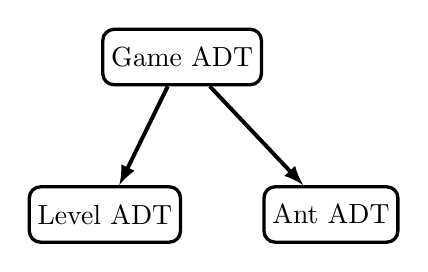
\begin{tikzpicture}[-latex, line width=0.5mm, >=stealth']

 % Position of GAM 
 % Use previously defined 'state' as layout (see above)
 % use tabular for content to get columns/rows
 % parbox to limit width of the listing
 \node[state] (GAM) 
 { Game ADT };
  
 % State: LEV with different content
 \node[state,    	% layout (defined above)
  below of=GAM, 	% Position is to the right of GAM
  node distance=2cm, 	% distance to GAM
  anchor=east] (LEV) 	% posistion relative to the center of the 'box'
	{Level ADT};

 \node[state,    	% layout (defined above)
  right of=LEV, 	% Position is to the right of GAM
  node distance=2cm, 	% distance to GAM
  anchor=west] (ANT) 	% posistion relative to the center of the 'box'
	{Ant ADT};

 \path 
	 (GAM) 	edge 	node[anchor=east,below]{} (ANT)
	 (GAM)	edge  node[anchor=west,below]{} (LEV);
\end{tikzpicture}
\end{center}


\chapter{Planning}
...


\end{document}

\message{ !name(VoorstudieFase1.tex) !offset(-78) }
